\documentclass{handout_utfpr}

\usepackage{xspace}
\usepackage{pbox}
\usepackage[brazil]{babel}
\usepackage{xcolor}
\definecolor{dark-gray}{gray}{0.20}
\definecolor{light-gray}{gray}{0.85}

\newcommand{\com}[1]{
\colorbox{light-gray}{\texttt{\pbox{\textwidth}{\$ #1}}}
}

\newcommand{\cominline}[1]{
\colorbox{light-gray}{\texttt{\pbox{\textwidth}{#1}}}
}

\handoutdate{\today}

\begin{document}
\maketitle
\section{Introdução}

Este material é apresentado como parte de uma série de minicursos que serão ministrados sobre tópicos variados com o intuito de \textit{nivelar} o conhecimento dos alunos com relação a conceitos básicos que não estão inclusos nas ementas das disciplinas regulares do curso, bem como colocá-los em contato com ferramentas úteis e boas práticas da Computação.

Os conteúdos são dispostos aqui apenas como um apanhado geral com o objetivo de prover um embasamento mínimo e recomenda-se que outras fontes de pesquisa sejam utilizadas para o aprofundamento nestes assuntos.

\subsection{Unix}
O sistema \textbf{Unix} é um sistema operacional desenvolvido por Ken Thompson, Dennis Richie, Douglas McIlroy e Joe Ossanna em 1970, na American Telephone \& Telegraph Company (AT\&T).

Este sistema foi projetado para ser portável, multi-tarefa e multi-usuário. Sistemas Unix são caracterizados por vários conceitos, como o uso de arquivos de texto para guardar dados, um sistema de arquivos hierárquico, o tratamento de certos dispositivos como arquivos e a idéia de que é melhor ter vários programas pequenos, cada um desempenhando uma única tarefa, de forma que eles possam ser encadeados para realizar uma tarefa maior do que o uso de um só programa que possua todas as funcionalidades. Estes conceitos são conhecidos como a ``filosofia Unix''.

% que permitia uma grande portabilidade para diversas plataformas, o que fez com que o sistema crescesse rapidamente e fosse muito utilizado por instituições academicas. O sistema Unix gerou a criação do projeto GNU por Richard Stallman.

% Under Unix, the operating system consists of many utilities along with the master control program, the kernel. The kernel provides services to start and stop programs, handles the file system and other common "low level" tasks that most programs share, and schedules access to avoid conflicts when programs try to access the same resource or device simultaneously. To mediate such access, the kernel has special rights, reflected in the division between user-space and kernel-space.

\subsection{Tanenbaum e o MINIX}
Em 1987, Andrew S. Tanenbaum, enquanto professor da Vrije Universiteit em Amsterdã, desenvolveu o \textbf{MINIX} (mini-Unix), um sistema que seguia os mesmos princípios do Unix mas que seria usado somente propósitos educacionais, como material de apoio ao seu livro ``Operating Systems: Design and Implementation'' (em português: ``Sistemas Operacionais: Projeto e Implementação'').

Os princípios aplicados por Tanenbaum no MINIX, influenciaram um de seus alunos, Linus Torvalds quando da criação de seu próprio sistema operacional, que mais tarde se tornaria o \textit{kernel} do \textbf{Linux}.

% No final do desenvolvimento de seu sistema, Linus compartilhou em um fórum o que havia feito:

% \emph{Hello everybody out there using minix -
% I'm doing a (free) operating system (just a hobby, won't be big and professional like gnu) for 386(486) AT clones. This has been brewing since april, and is starting to get ready. I'd like any feedback on things people like/dislike in minix, as my OS resembles it somewhat (same physical layout of the file-system (due to practical reasons) among other things).

% I've currently ported bash(1.08) and gcc(1.40), and things seem to work. This implies that I'll get something practical within a few months, and I'd like to know what features most people would want. Any suggestions are welcome, but I won't promise I'll implement them :-)
% Linus (torvalds@kruuna.helsinki.fi)

% PS. Yes – it's free of any minix code, and it has a multi-threaded fs. It is NOT portable (uses 386 task switching etc), and it probably never will support anything other than AT-harddisks, as that's all I have :-(.

% —Linus Torvalds}

\section{Conhecendo o Linux}

\subsection{GNU/Linux}
Embora a maioria das pessoas conheça apenas o termo Linux, a nomenclatura mais acurada para o sistema que se usa nos dias de hoje é ``GNU/Linux''. Isso se dá devido ao fato de que a maioria das distribuições Linux (vide \ref{distro}) na verdade contêm o \textit{kernel} (vide \ref{kernel}) do Linux em conjunto com \textit{softwares} GNU.

O projeto GNU foi iniciado em setembro de 1983 por Richard Stallman, enquanto trabalhava no laboratório de inteligência artificial do Massachusetts Institute of Technology (MIT). O intuito do projeto é criar um ambiente de colaboração em que usuários de computadores possam ter acesso a programas que são distribuídos juntamente com o seu código-fonte (\textit{software} livre). A idéia da disseminação do \textit{software} livre é dar aos seus usuários total controle sobre os programas que são utilizados, ao contrário do \textit{software} proprietário, em que é provido o executável, mas não há como realizar modificações, nem mesmo saber o conteúdo do código que gerou o mesmo.

Juntamente com o projeto GNU, foi criado o movimento ``Free software'' e a instituição de fins não lucrativos ``Free software foundation'', que atualmente, entre outras atividades, administra o projeto GNU e as licenças GNU.

\subsection{O kernel}\label{kernel}
O \textit{kernel} é a parte do sistema que faz a ponte entre os recursos de \textit{hardware}, como memória, CPU, dispositivos de entrada e saída; e a camada de \textit{software}.

Numa configuração monolítica (Linux, Windows, etc), os programas rodam em ``espaço de usuário'', o que significa que um programa usa apenas o espaço de memória reservado a ele e não possui acesso direto a recursos do sistema. Para que um programa efetue uma ação como por exemplo exibir uma mensagem na tela, é necessário que uma ``chamada de sistema'' seja feita através do \textit{kernel}, já que o programa não tem acesso à placa gráfica do computador.

A figura a seguir exemplifica a arquitetura básica de um sistema Linux:
\begin{figure}[!h]
  \centering
  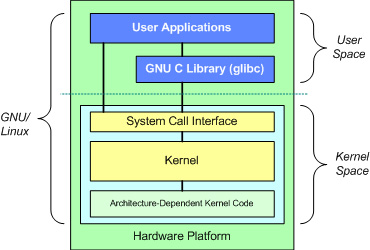
\includegraphics[scale=.8]{kernel.jpg}
  \caption{Arquitetura de um sistema GNU/Linux}
  \label{fig:kernel}
\end{figure}
Na camada superior, em espaço de usuário, estão as aplicações de usuário e a biblioteca GNU. Estas aplicações interagem com o \textit{kernel} através de uma interface de chamadas de sistema. O \textit{kernel}, por sua vez, faz acesso ao hardware.

\subsection{Distribuições}\label{distro}
Como visto anteriormente, o que se conhece popularmente como Linux, é na verdade apenas o \textit{kernel}. Então, para que possamos ter um sistema funcionando, é necessário fazer a escolha de uma ``distribuição''. Distribuições nada mais são que o \textit{kernel} do Linux juntamente com alguns outros \textit{softwares} (em sua maioria GNU, mas não necessariamente) que dão funcionalidade ao sistema.

Algumas distribuições mais comuns são: Ubuntu, Debian, Fedora, entre várias outras.

O conceito de distribuição (também chamadas de ``distro'') geralmente gera alguma confusão entre os usuários de Linux, já que todos os softwares com os quais a pessoa está interagindo no uso cotidiano do sistema são na verdade softwares que são providos pela distribuição. Isto faz com que um usuário, ao experimentar várias distros em seu computador, não perceba que na verdade, o \textit{kernel} rodando por baixo da camada de software de usuário é o mesmo para todas as distribuições.

\subsubsection{Desktop Environments e Window Managers}
Outra distinção importante que deve ser feita é quanto ao conceito de Desktop Environments (ambientes de desktop) e Window Managers (gerenciadores de janelas). Falando de maneira grosseira, Desktop Environments são a parte da distribuição responsável por partes do sistema como o ``menu iniciar'', gerenciamento de sessão e o próprio desktop. Os Window Managers são a parte que gerencia a aparência das janelas e o comportamento de funções como a troca de janelas (alt + Tab).

A maioria das distribuições já provê um DE e um WM, porém algumas delas trazem apenas os programas essenciais, ficando a instalação da parte gráfica a cargo do usuário. É importante entender a diferença entre distro, desktop environment e window manager para que no caso de um problema ou caso alguma funcionalidade não lhe agrade, você saiba exatamente em qual parte do sistema está o problema.

\section{Como obter?}
A maioria das distribuições Linux é disponibilizada grátis na internet na forma de imagens \textit{.iso}. Para a instalação, as seguintes alternativas existem:

\begin{enumerate}
\item Manter o sistema operacional nativo e rodar Linux em uma máquina virtual\\
  Recomendado para testes iniciais, antes de se decidir por uma distribuição.
  
\item Manter o sistema operacional nativo e o Linux em dual-boot\\
  Recomendado para aqueles que usam com frequência as funcionalidades do sistema nativo, como jogos ou softwares proprietários não disponíveis para Linux.
  
\item Remover o sistema nativo e usar somente Linux\\
  Recomendado para aqueles que já tem certa experiência com Linux e não necessitam de outro sistema operacional.
  
\item Trocar o sistema nativo pelo Linux e rodar o sistema antigo em uma máquina virtual\\
  Para aqueles que já optaram por usar Linux, mas que em uma pequena fração do tempo, ainda precisam de funcionalidades do outro sistema.
\end{enumerate}

\subsection{Máquina Virtual}

Uma máquina virtual (\textbf{VM}) é, como o nome indica, um computador virtual baseado somente em \emph{software} que funciona como um emulador, reproduzindo a arquitetura e funcionalidades de um computador de verdade. Através da máquina virtual, pode-se ter vários sistemas operacionais instalados em uma mesma máquina e utilizá-los todos sem afetar o sistema base do computador.

\begin{figure}[!h]
  \centering
  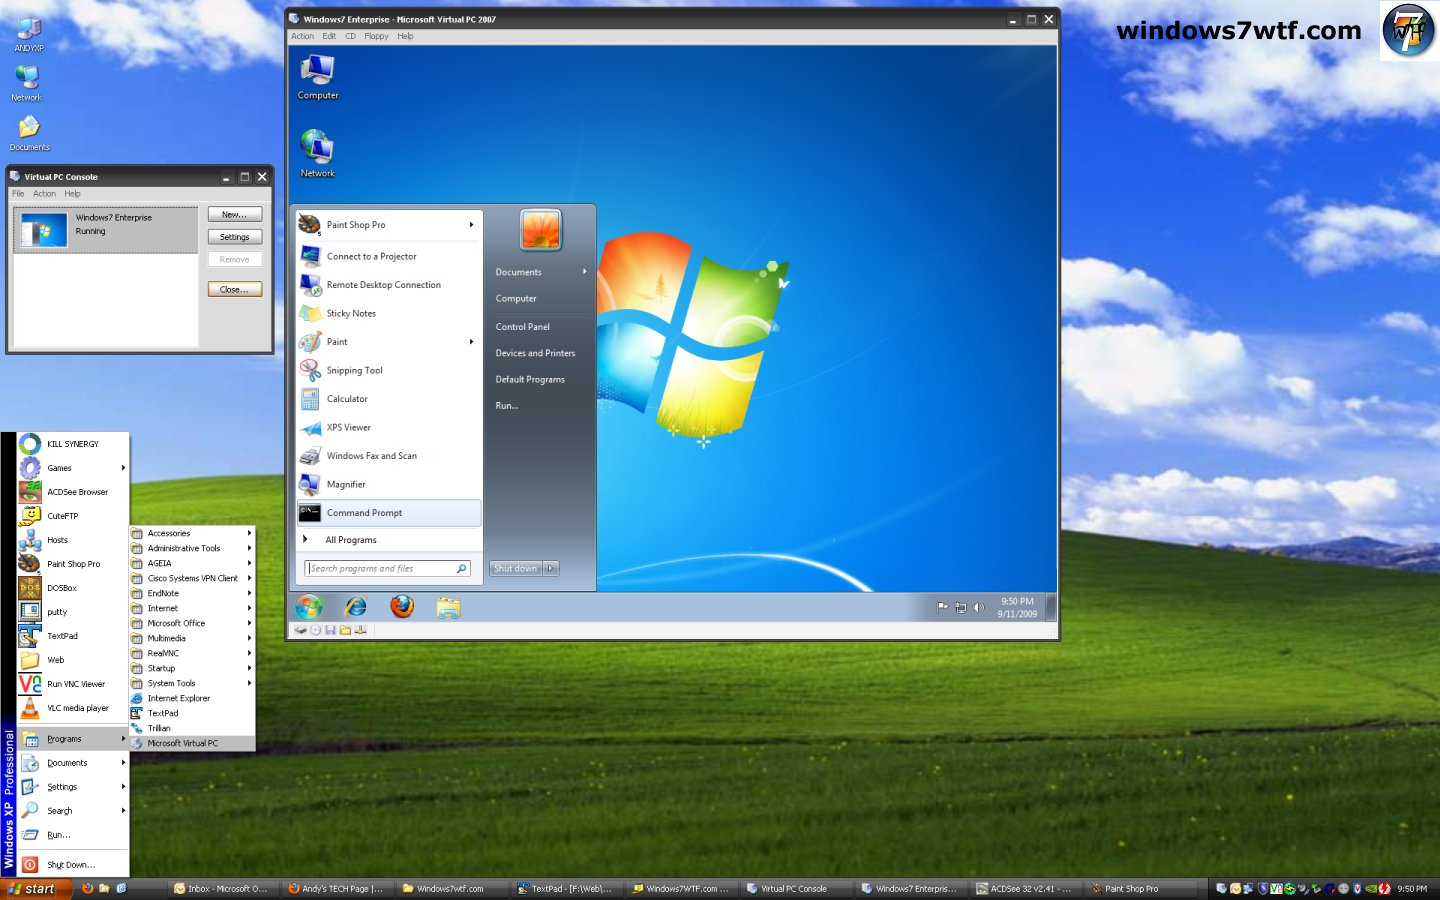
\includegraphics[scale=.3]{vm.jpg}
  \caption{Exemplo do uso de uma máquina virtual}
  \label{fig:vm}
\end{figure}

Observe a imagem \ref{fig:vm} acima. Nela pode-se ver um sistema Windows servindo como base para outro sistema Windows rodando dentro da VM. O sistema que está dentro da VM não afeta de maneira alguma o sistema base. Desta forma, já que a VM nada mais é que um \textit{software} rodando em um sistema qualquer, podemos levantar as seguintes vantagens de seu uso:

\begin{itemize}
\item Nada que seja feito no sistema virtual afetará o sistema real.
\item Pode-se instalar e desinstalar vários sistemas com facilidade.
\item Em situações em que o sistema base possui acesso restrito, como em um ambiente acadêmico, a VM pode ser uma boa alternativa, já que dentro da máquina virtual o usuário possui controle total.
\end{itemize}

Porém, pelo mesmo fato de ser apenas um programa rodando em seu computador a VM tem as desvantagens de que:

\begin{itemize}
\item Como estão sendo utilizados recursos de um sistema para rodar outro sistema, ocorrerá diminuição da eficiência, e o sistema poderá ficar lento ou não ter memória suficiente para executar algum programa.
  \item Para uma utilização prolongada, será sempre melhor instalar o sistema diretamente em seu computador.
\end{itemize}  

\subsection{Dual-boot}
Outra alternativa bastante popular na instalação de sistemas operacionais é o dual-boot, ou multi-boot. Nessa situação, os dois (ou mais) sistemas serão instalados totalmente em uma máquina, cada qual recebendo uma porção do disco rígido. Quando o usuário liga o computador, uma tela é exibida permitindo que se escolha qual dos sistemas deve ser carregado. Para alternar entre sistemas, basta reiniciar o computador e escolher o outro sistema.

A principal vantagem dessa abordagem é que ambos os sistemas possuem a máquina toda para si, exatamente como ocorre quando há apenas um sistema operacional instalado.

Uma desvantagem que pode ser citada é que não é possível executar os dois sistemas ao mesmo tempo e deve-se aguardar o \textit{reboot} para selecionar o outro sistema.

\section{Porque usar?}
Existem algumas características dos sistemas baseados em Linux que fazem com que eles sejam atrativos para o uso na Ciência da Computação. Pode-se dizer que um sistema Linux possui foco nos desenvolvedores de sistemas enquanto que outros sistemas operacionais possuem foco no usuário.

\subsection{Familiaridade geral com termos e conceitos}
Pelo fato de se basear em software de código aberto, existem muitos conceitos teóricos da computação que podem ser verificados muito facilmente quando se usa Linux. Um exemplo simples é o próprio \textit{kernel}, que é escrito na linguagem C. Ao estudar programação ou Sistemas Operacionais, o código do \textit{kernel} pode ser explorado para que se entenda como os conceitos estudados são aplicados em um sistema operacional ``de verdade''.

Outro exemplo são as aplicações na área de Redes de Computadores que em sua maioria se baseiam em Linux. Ao usar Linux no seu dia a dia, você já estará se familiarizando com alguns conceitos nesta área.

\subsection{Aprendizado de boas práticas}
O uso contínuo do sistema pode levar ao conhecimento de boas práticas de programação. Um bom exemplo é a ``filosofia'' de se projetar programas que façam apenas uma tarefa, mas a façam de maneira bem feita.

Outro ponto que se pode ressaltar é o fato de o Linux ser bastante documentado. Isso significa que os programas possuem um manual de instruções de utilização. Acosutmar-se a ler manuais e pesquisar sobre funções desconhecidas é um ponto importante dentro da computação, já que constantemente nos deparamos com código escrito por outras pessoas ou situações novas nas quais não possuímos domínio. Saber buscar informação nos lugares certos é algo valioso.

\subsection{Gerenciamento de pacotes}
Além dos benefícios dentro da computação, as distribuições Linux também trazem algumas funcionalidades que são úteis para qualquer pessoa. O gerenciamento de pacotes é uma delas.

Normalmente, as distribuições Linux aplicam o conceito de ``pacote''. Um pacote nada mais é que um programa preparado para ser instalado em seu sistema. Pacotes são específicos para cada distribuição e garantem que programas serão instalados e desinstalados de forma correta. Além disso, há o conceito de ``repositórios'' que são servidores que abrigam vários pacotes. A vantagem dessa abordagem é que quando se quer instalar um programa, ao invés de se procurar em um site de busca pelo programa que se deseja, baixar um executável e instalar o programa; um usuário Linux pode simplesmente digitar o nome do programa em seu gerenciador de pacotes que irá automaticamente percorrer os repositórios procurando pelo pacote correto, mais atual e com garantia de idoneidade. Isto mantém o sistema muito fácil de gerenciar, já que o gerenciador de pacotes toma conta de tudo. Os pacotes também são, em geral, submetidos ao julgamento da comunidade de usuários do sistema, tornando pacotes ``quebrados'' ou com código malicioso mais difíceis de serem encontrados.

\section{Uso da linha de comando}

Quando utilizamos um computador, estamos acostumados a usar a \underline{interface gráfica}. Isso significa que fazemos bastante uso do mouse para acessar as variadas funções do sistema e os resultados das nossas ações são exibidos na tela de maneira muito clara. Ex: ao mover um arquivo, podemos simplesmente clicar sobre ele e arrastá-lo para outra pasta. Esta interação é feita de maneira muito intuitiva.

Embora hoje em dia, quase todas as distribuições Linux possuam uma interface gráfica, o seu ponto forte é a \underline{interface de linha de comando}. A CLI (\emph{Command Line Interface}) não é baseada nos preceitos de mouse + gráficos com os quais estamos acostumados. A sua utilização se faz através de comandos de texto. Para realizar tarefas como a criação de uma pasta, ou fazer a cópia de um arquivo, um comando será digitado em um console. Para executar a mesma ação do exemplo anterior, digitaríamos o comando: \com{mv local\_arquivo local\_destino}. O comando não retornaria resposta alguma, o que em um sistema Unix significa que tudo ocorreu com sucesso. No começo, esta nova forma de interagir com o computador e estes comandos podem parecer intimidantes, porém com o tempo e costume, a utilização da CLI fará com que a navegabilidade se torne rápida e focada.

Além da navegação básica pelas pastas, os comandos da CLI também podem ser combinados de forma a executar tarefas complexas, como manipulação de arquivos, gerenciamento de rede, atividades que em outros sistemas operacionais provavelmente teríamos que procurar por um programa na internet para realizá-las.

A seguir, veremos alguns comandos básicos e sua utilização.



% Um comando da CLI possui um nome e pode possuir parâmetros. Esses parametros podem modificar o comportamento do comando para suprir as suas necessidades. Normalmente, um parâmetro acompanha o nome do comando dessa forma: \cominline{grep -h}, onde ``h'' pode ser a forma abreviada de um parâmetro. É comum a forma mais longa ser acompanhada de dois ``-'', da seguinte forma: \cominline{grep --help}. Informações sobre os parâmetros podem ser encontradas no manual do comando, assim como sua descrição e exemplos de uso. O manual é acessado dessa maneira: \cominline{man grep}.
% \\

Como um guia, todas as linhas de comandos terão o caracter \$ no começo, apenas para indicar a linha onde será digitado o comando em questão. O caracter não faz parte do comando e deve ser ignorado.\\

Ao abrir uma janela de terminal, primeiramente precisamos saber ``onde estamos''. Para saber em qual pasta você está trabalhando na linha de comando, digite \textbf{pwd}, que significa ``print working directory''.\\

\com{pwd\\/home/usuario}\\

A resposta do comando é a pasta atual. ``/home/usuario'', seria similar ao ``C:\textbackslash Usuários\textbackslash usuário\textbackslash'' \  de um sistema Windows.

Há alguns ``atalhos'' que podem ser utilizados na hora de digitar comandos:
\begin{itemize}
\item o caracter \textbf{$\sim$} é uma outra forma de representar a pasta ``/home/usuario''  
\item um \textbf{.} significa o diretório atual e \textbf{..} é equivalente ao diretório anterior. Portanto, no caso acima, \textbf{.} significaria ``/home/usuario'' e \textbf{..} significaria ``/home''
\end{itemize}
A mudança de diretórios, ou seja, pastas, deve ser feita através do comando \textbf{cd} (``change directory'').

\com{cd /home/usuario/Área\textbackslash\xspace de\textbackslash\xspace Trabalho/\\\$ cd ..\\\$ pwd\\/home/usuario\\\$ cd ./Área\textbackslash\xspace de\textbackslash\xspace Trabalho/\\\$ pwd\\/home/usuario/Área\textbackslash\xspace de\textbackslash\xspace Trabalho}\\

É importante lembrar que o / também é um diretório! Esta é a pasta raiz do seu sistema, portanto:\\

\com{cd /home/usuario/}
é \underline{\textbf{diferente}} de:
\com{cd home/usuario/}\\

Você pode criar uma pasta usando o \textbf{mkdir} (``make directory''). Lembre-se que sempre que você não souber em que pasta você está, você pode utilizar o pwd.\\

\com{cd /tmp/\\\$ mkdir NovaPasta\\\$ mkdir NovaPasta/Pasta2}\\

Se você desejar saber o conteúdo de uma pasta, basta utilizar o comando \textbf{ls} (``list''). Este comando mostrará tanto pastas quanto arquivos presentes.\\

\com{cd /tmp/\\\$ ls\\NovaPasta\\\$ cd NovaPasta\\\$ ls\\Pasta2}\\

Para remover uma pasta, um simples comando pode ser usado, o \textbf{rmdir}, porém a pasta só será removida se ela estiver vazia, caso contrário uma mensagem de erro aparecerá na tela. No nosso exemplo, podemos excluir a Pasta2 dessa forma:\\

\com{cd /tmp/\\\$ rmdir ./NovaPasta/Pasta2}\\

Você pode criar um arquivo vazio com apenas um comando, o \textbf{touch}. \\

\com{cd /tmp/NovaPasta\\\$ touch teste.txt}\\

Para podermos copiar um arquivo, utilizaremos o comando \textbf{cp}.\\

\com{ls /tmp/NovaPasta\\teste.txt\\\$ cp /tmp/NovaPasta/teste.txt /tmp/teste2.txt}\\

Utilizando o \textbf {cp} com o parâmetro \textbf{-r} somos capazes de copiar pastas.\\

\com{cp -r /tmp/NovaPasta /tmp/NovaPasta2}\\

Remover um arquivo definitivamente é bem simples quando utilizamos o comando \textbf{rm}. Apenas é necessário colocar o nome do arquivo que se deseja excluir e estar na pasta correta.\\

\com{cd /tmp/\\\$ rm teste2.txt}\\

Novamente, para excluirmos uma pasta, é preciso usar o parâmetro \textbf{-r}. É preciso ter muito cuidado ao usar essa funcionalidade, pois esse comando apagará definitivamente qualquer pasta mesmo que haja conteúdo dentro.\\

\com{cd /tmp/\\\$ rm -r NovaPasta2}\\
\\

Há outros comandos que são interessantes:
\begin{itemize}
\item\cominline{cat ArquivoQualquer.txt} - Imprime na tela o conteúdo de ArquivoQualquer.txt
\item\cominline{find /home/usuario -name ArquivoQualquer} - Procura dentro da ``home'' um arquivo de nome ArquivoQualquer.
\item\cominline{grep string caminho\_para\_pasta/} - Procura dentro dos arquivos da pasta a string colocada após grep.
\item\cominline{shutdown -h now} - Desliga o computador.
\item\cominline{shutdown -r now} - Reinicia o computador.
\item\cominline{sudo comando} - Executar um programa como um super usuário.
\item\cominline{tar -cf Arquivo.tar.gz caminho\_para\_pasta/} - Comprimir arquivos na pasta indicada pelo caminho.
\item\cominline{tar -xf Arquivo.tar.gz} - Extrair arquivos de um .tar.gz.
\end{itemize}

\end{document}










